\section{Experimental Results}
\label{sec:exp}
\subsection{Evaluation on Workloads}
The experiments were conducted on two different systems. First, a CPU-based system equipped with an Intel Xeon E3-1245 running 4 cores at 3.4\,Ghz and 24\,GB main memory. Second a MIC, the Intel Xeon Phi 7120P which has 60 cores with 4 hyper-threads, each clocked at 1.23\,Ghz. It also has 16\,GB main memory with a bandwidth of 352\,GB/s. To allow a comparison, the experiment parameters used were the same on both platforms. For each experiment five iterations were averaged and their standard deviation was computed.

Three types of workload were executed, \textit{mixed}, \textit{push} and \textit{pop}. For the mixed and pop, the concurrent priority queue was prepopulated with 1000$\times$threads in the former and 10\,Mio. elements in the latter. Prepopulation was not included in the measured runtime. The \textit{mixed} workload chooses for each operation with a probability of 50\% either a \textit{push} or \textit{pop} operation. The number of threads is increased from 1 to 240, in steps of 20, while the number of operations per threads stays constant.

\subsubsection{Evaluation on Xeon Haswell}
\begin{figure*}[t]
	\centering
	\begin{subfigure}[b]{0.3\textwidth}
		\centering
		%\includegraphics[width=\textwidth]{../plots/i7_mixed/runtime_mixed_i7}
		\input{../plots/xeon_mixed/xeon_mixed}
		\caption{Mixed workload}
		\label{fig:xeon_mixed}
	\end{subfigure}
	\hfill
	\begin{subfigure}[b]{0.3\textwidth}
		\centering
		\input{../plots/xeon_push/xeon_push}
		\caption{Push workload}
		\label{fig:xeon_push}
	\end{subfigure}
	\hfill
	\begin{subfigure}[b]{0.3\textwidth}
		\centering
		%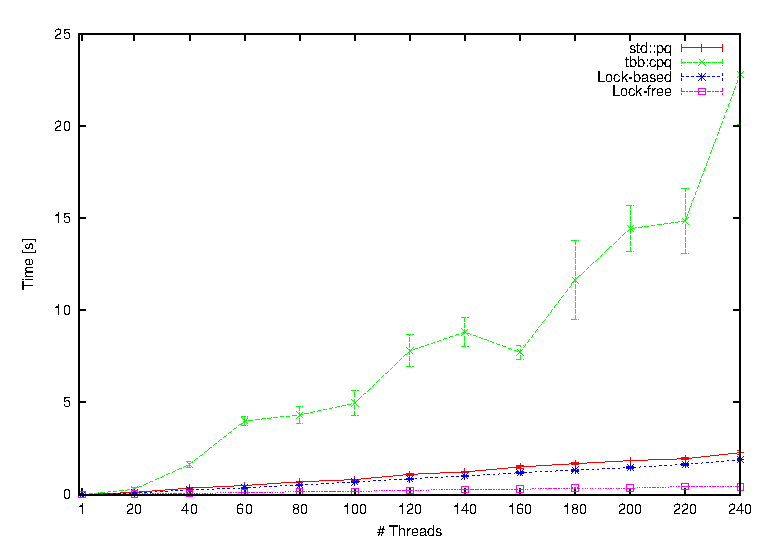
\includegraphics[width=\textwidth]{../plots/i7_pop/runtime_pop_i7}
		\begin{tikzpicture}
\begin{axis}[
width=2.5in,
xlabel={\#Threads},
ylabel={Time [s]},
xmin=-10,
xmax=250,
xtick={0,80,...,240},
ytick={0, 500, 1000, 1500},
yticklabels={0, 0.5, 1, 1.5},
ymin=0,
ymax=1500,
scaled x ticks = false,
y label style={at={(0.1,0.5)}},
legend style={at={(0.05,0.95)},anchor=north west, font=\tiny}]

\addplot[mark=*,blue, mark size=1.5]
table[x=Threads,y=std,col sep=comma] {../plots/xeon_pop/xeon_pop.csv}; 
\addlegendentry{std::pq}

\addplot[color=red,mark=triangle*, mark size=2]
table[x=Threads,y=tbb,col sep=comma] {../plots/xeon_pop/xeon_pop.csv}; 
\addlegendentry{tbb::cpq}

\addplot[color=brown,mark=square*, mark size=1.5]
table[x=Threads,y=lb,col sep=comma] {../plots/xeon_pop/xeon_pop.csv}; 
\addlegendentry{Lock-based}

\addplot[color=darkgreen,mark=diamond*, mark size=2]
table[x=Threads,y=lf,col sep=comma] {../plots/xeon_pop/xeon_pop.csv}; 
\addlegendentry{lock-free}

\end{axis}
\end{tikzpicture}
		\caption{Pop workload}
		\label{fig:xeon_pop}
	\end{subfigure}
	\caption{Runtime for different workloads executed on a Xeon E3-1245 while varying the number of threads}
	\label{fig:eval_i7}
\end{figure*}
Fig.~\ref{fig:eval_i7} shows the run-times for executing the three workloads on a Xeon E3-1245 system. All variants are performing and behaving similar in the \textit{mixed} and \textit{push} workload, except for the lock-based implementation which struggles more to scale with the number of threads. Our lock-free implementation is very close to the baseline implementations and shows similar behavior when increasing the number of threads. In the pop workload, all four data structures behave very similar.
The lock-free implementation with a \textit{pop} operation in $\Theta(1)$ and lazy-deletion shows the best runtime by a small margin.

\subsubsection{Evaluation on Xeon Phi}
\begin{figure*}[t]
	\centering
	\begin{subfigure}[b]{0.3\textwidth}
		\centering
		%\includegraphics[width=\textwidth]{../plots/xp_mixed/runtime_mixed}
		\begin{tikzpicture}
\begin{axis}[
width=2.5in,
xlabel={\#Threads},
ylabel={Time [s]},
xmin=-10,
xmax=250,
xtick={0,80,...,240},
ytick={0,10000, 20000, 30000},
yticklabels={0, 10, 20, 30},
ymin=0,
ymax=30000,
scaled x ticks = false,
scaled y ticks = false,
y label style={at={(0.1,0.5)}},
legend style={at={(0.05,0.95)},anchor=north west, font=\tiny}]

\addplot[mark=*,blue, mark size=1.5]
table[x=Threads,y=std,col sep=comma] {../plots/xp_mixed/xp_mixed.csv}; 
\addlegendentry{std::pq}

\addplot[color=red,mark=triangle*, mark size=2]
table[x=Threads,y=tbb,col sep=comma] {../plots/xp_mixed/xp_mixed.csv}; 
\addlegendentry{tbb::cpq}

\addplot[color=brown,mark=square*, mark size=1.5]
table[x=Threads,y=lb,col sep=comma] {../plots/xp_mixed/xp_mixed.csv}; 
\addlegendentry{Lock-based}

\addplot[color=darkgreen,mark=diamond*, mark size=2]
table[x=Threads,y=lf,col sep=comma] {../plots/xp_mixed/xp_mixed.csv}; 
\addlegendentry{lock-free}

\end{axis}
\end{tikzpicture}
		\caption{Mixed workload}
		\label{fig:xp_mixed}
	\end{subfigure}
	\hfill
	\begin{subfigure}[b]{0.3\textwidth}
		\centering
		%\includegraphics[width=\textwidth]{../plots/xp_push/runtime_push}
		\begin{tikzpicture}
\begin{axis}[
width=2.5in,
xlabel={\#Threads},
ylabel={Time [s]},
xmin=-10,
xmax=250,
xtick={0,80,...,240},
ytick={0, 15000, 30000, 45000, 60000},
yticklabels={0, 15, 30, 45, 60},
ymin=0,
ymax=60000,
scaled x ticks = false,
scaled y ticks = false,
y label style={at={(0.1,0.5)}},
legend style={at={(0.05,0.95)},anchor=north west, font=\tiny}]

\addplot[mark=*,blue, mark size=1.5]
table[x=Threads,y=std,col sep=comma] {../plots/xp_push/xp_push.csv}; 
\addlegendentry{std::pq}

\addplot[color=red,mark=triangle*, mark size=2]
table[x=Threads,y=tbb,col sep=comma] {../plots/xp_push/xp_push.csv}; 
\addlegendentry{tbb::cpq}

\addplot[color=brown,mark=square*, mark size=1.5]
table[x=Threads,y=lb,col sep=comma] {../plots/xp_push/xp_push.csv}; 
\addlegendentry{Lock-based}

\addplot[color=darkgreen,mark=diamond*, mark size=2]
table[x=Threads,y=lf,col sep=comma] {../plots/xp_push/xp_push.csv}; 
\addlegendentry{lock-free}

\end{axis}
\end{tikzpicture}
		\caption{Push workload}
		\label{fig:xp_push}
	\end{subfigure}
	\hfill
	\begin{subfigure}[b]{0.3\textwidth}
		\centering
		%\includegraphics[width=\textwidth]{../plots/xp_pop/runtime_pop}
		\input{../plots/xp_pop/xp_pop}
		\caption{Pop workload}
		\label{fig:xp_pop}
	\end{subfigure}
	\caption{Runtime for different workloads executed on a Xeon Phi while varying the number of threads}
	\label{fig:eval_xp}
\end{figure*}
The same workloads were also run on Xeon Phi. The measured run-times are plotted in Fig.~\ref{fig:eval_xp}.
In the mixed workload the TBB and the lock-free concurrent priority queue behave similarly well. The other two implementations show clearly a longer runtime.
%FIXME WHAT IS rsp?
Looking at the \textit{push} rsp. \textit{pop} workload it is visible that the longer runtime in the lock-based implementation originates from bad performance for the \textit{push} operation, while for the STD implementation the \textit{pop} operation is the cause for the long runtime.
The TBB implementation behaves well in all three workloads.
Our lock-free implementation shows almost the same behavior with a slightly longer runtime.

Comparing the runtime of the two platforms shows that the same workload is about one magnitude faster on Xeon CPU.

%Implementing a truly concurrent data structure is a challenging task for many reasons. For instance, even though our implementation is lock-free, it may not be starvation-free. There could be a thread A that when going through the lowest level of the skip list searching for the next un-marked node (i.e. logically undeleted) gets always outrun by some other thread B. This means that thread A can fail repeatedly if the others threads always succeed. Moreover, thread contention may happen if many threads try to logically delete a node (i.e. mark a node). Only one thread will succeed and all the other unsuccessful ones will race to mark  the next available node. 
%Another problem could arise when some node physically deletes a node that other threads are still using. This will lead into repeated \textit{compareAndSet} failures.

\subsection{Impact of cache-invalidation}
\begin{figure}[t]
	\centering
	%\includegraphics[width=0.9\columnwidth]{../plots/comp_contains/runtime_contains}
	\begin{tikzpicture}
\begin{axis}[
width=2.7in,
xlabel={\#Threads},
ylabel={Time [s]},
xmin=-10,
xmax=250,
xtick={0,80,...,240},
ytick={0,2000, 4000, 6000, 8000, 10000},
yticklabels={0, 2, 4, 6, 8, 10},
ymin=0,
ymax=10000,
scaled x ticks = false,
scaled y ticks = false,
legend style={at={(0.05,0.95)},anchor=north west, font=\tiny}]

\addplot[mark=*,blue, mark size=1.5]
table[x=Threads,y=lf_xeon,col sep=comma] {../plots/comp_contains/comp_contains.csv}; 
\addlegendentry{Xeon E-1245}

\addplot[color=red,mark=triangle*, mark size=2]
table[x=Threads,y=lf_i7,col sep=comma] {../plots/comp_contains/comp_contains.csv}; 
\addlegendentry{Core i7-3820}

\addplot[color=darkgreen,mark=square*, mark size=1.5]
table[x=Threads,y=lf_xp,col sep=comma] {../plots/comp_contains/comp_contains.csv}; 
\addlegendentry{Xeon Phi}

\end{axis}
\end{tikzpicture}
	\caption{Cache-invalidation assessment}
	\label{fig:comp_contains}
\end{figure}
The previous experiments show that the same workload performs roughly a magnitude better on a Xeon CPU than on Xeon Phi.
Despite the fact that Xeon Phi has many more cores and a higher memory bandwidth.
While there are multiple reasons for this, e.g. different caching architecture, clock frequency, number of write buffers and so on, this experiment should evaluate the impact of cache-invalidation.
% FIXME: multiple reasons before, multiple reasons again... what is going wrong?
There are multiple reasons for these, e.g. cache structure, memory allocation cost, and other problems.
Therefore an experiment was designed to check how Xeon Phi performs, in comparison to other architectures when cache-invalidations are not occurring.
This consists of prepopulating our lock-free concurrent priority queue with 10 million elements, then each thread will do 100'000 lookups in the data structure.
Thereby the structure of the priority queue is unaltered which means no cache-line belonging to the concurrent priority queue should get invalidated.
This experiment was executed with 1 to 240 threads, the run-times, running this experiment on an Intel Core i7-3820, a Xeon CPU and the Xeon Phi, are plotted in Fig.~\ref{fig:comp_contains}.
% FIXME can you improve the second part of the following sentence. It should become 2 sentences, instead of 1.
It can be noted that the runtime on Xeon Phi stays stable up to 60 threads equaling the number of cores, with even more threads it increases only slightly.
Whereas on the other two systems, the execution time increases linearly.
The results show clearly that the invalidation of cache-lines and their consequences have a major impact on the performance on Xeon Phi.
While in the previous experiments it showed a linear increase in execution time when scaling up, in this one the runtime stays almost constant which is close to ideal.

%Also rephrase reson why Xeon Phi is not doing well
This finding is not new, other researchers~\cite{ramos-hoefler-cc-modeling} have shown that a drawback when using a Xeon Phi is that any cache-line invalidation might lead to many cores ending up with dirty cache lines. This is due to fact that it uses a distributed tag directory. Thus, the more hardware cores are used on a concurrent application the probability that at least two threads share a cache line is higher. These dirty cache lines produce expected overhead due to cache invalidations.

Implementing a truly concurrent data structure is a challenging task for many reasons. For instance, even though our implementation is lock-free, it may not be starvation-free. There could be a thread A that when going through the lowest level of the skip list searching for the next un-marked node (i.e. logically undeleted) gets always outrun by some other thread B. This means that thread A can fail repeatedly if the others threads always succeed. Moreover, thread contention may happen if many threads try to logically delete a node (i.e. mark a node). Only one thread will succeed and all the other unsuccessful ones will race to mark
the next available node.\\

\subsection{Operational intensity in different microarchitectures}
% recap of operational intensity ~\cite{roger1996science}
Operational intensity is defined as the ratio of the number of instructions executed to the number of memory accesses. If there exist many instructions per memory access, then the program is considered to have a high computational intensity i.e. compute bounded. On the other hand, if there are a small number of instructions are executed per memory access, then the program is considered to have a low computational intensity i.e. memory bounded.

% why we think it matters in our case
Our project goal was to design a simple, yet effective, concurrent priority queue. Thus, we expected to have an operational intensity dominated mainly by the number of memory accesses, and aimed to improve this. Having to move data around, has a different impact on different CPU architectures. We will describe and explain how our data structure behaves on Intel Haswell microarchitecture (Intel Core i7-4558U) and on Sandy BridgeE microarchitecture (Intel Core i7-3820K). 

% Differences between these two microarchitectures
The Intel Haswell microarchiteture is the successor of Ivy Bridge which in turn is the successor of Sandy Bridge. They have several differences but they also share many commonalities. One of the biggest change is the enhancement done on cache level operations. These changes are summarized in \tablename~\ref{tab:haswell_ivy}~\cite{ijcsit2013040321, microarchitecture, haswell_arch}.

%memory hierarchy implemented on the Intel Haswell. The cache bandwidth is doubled and its memory system can now perform two loads and one store per cycle. The Haswell's L1 load bandwidth is of 64 bytes/cycle, its L1 store bandwidth is of 32 bytes/cycle and also L2 bandwidth to L1 has doubled (from 32 bytes/cycle to 64 bytes/cycle). Other relevant improvements are the ones related to the Translation Look-aside Buffer (TLB) which in Haswell has access to 2M shared pages. The page entry also doubled in Haswell as well as the associativity; It went from a 4-way associative TLB in Ivy Bridge to a 8-way associative TLB in Haswell. 

\begin{table}[ht]
\footnotesize
\begin{tabular}{|l|l|l|ll}
\cline{1-3}
\multicolumn{1}{|c|}{\textbf{Metric}} & \multicolumn{1}{c|}{\textbf{Sandy BridgeE}} & \multicolumn{1}{c|}{\textbf{Haswell}} &  &  \\ \cline{1-3}
L1 Load Bandwidth                     & 32 Bytes/cycle                           & 64 Bytes/cycle                        &  &  \\ \cline{1-3}
L1 Store bandwidth                    & 16 Bytes/cycle                           & 32 Bytes/cycle                        &  &  \\ \cline{1-3}
L2 Bandwidth to L1                    & 32 Bytes/cycle                           & 64 Bytes/cycle                        &  &  \\ \cline{1-3}
L2 Unified TLB                        & 4K:512, 4-way                            & 4k+2M shared: 1024, 8-way             &  &  \\ \cline{1-3}
\end{tabular}
\caption{Cache operation differences between Intel Haswell and Intel SandyBridgeE}
\label{tab:haswell_ivy}
\end{table}

% describe cache structure
In addition to core cache size, latency, and bandwidth improvements, the Intel Haswell microarchitecture has also improved its ICache prefetch algorithms, and the way it handles conflicts. It uses hardware transactions, i.e. it uses hardware to keep track of which cache lines have been read from and which have been written to. L1 cache tracks addresses read/written from/to, respectively, in the transactional region and it may evict address but without loss of tracking. Data conflicts occur if at least one request is doing a write, but it is detected at cache line granularity and using existing cache coherence protocol.%~\cite{dk_haswell,rajwar_qconsf2012}

While running our priority queue benchmark on these two different architectures, we observed different behaviors. The running times when using an Intel IvyBridge processor dramatically increase due to a higher number of instructions and cache misses. Everytime we need to perform an insertion, we first have to search for the adequate place within the skip list. The average of the skip list nodes fit in a 64-byte cache line but the ones containing pointers in upper levels do not. On the other hand, when we used an Intel Haswell processor, running times were much less than in the Sandy BridgeE processor. This is mainly due to the improvements done on cache operations. In this case, our data structure can take advantage of such improvements by loading more skip list nodes into the caches that can also be used by other threads.

% explain data + graph + core architecture
\begin{figure}[t]
	\centering
  	%\includegraphics[scale=0.3]{../plots/haswell-ivybridge/haswell_ivybridge.pdf}
	\begin{tikzpicture}
\begin{axis}[
width=3in,
xlabel={Number of operations},
ylabel={Operations Intensity},
%xmin=-10,
%xmax=250,
xmode=log,
xtick={1, 100, 10000, 1000000},
ytick={0, 5, 10, 15, 20},
ymin=0,
ymax=20,
scaled x ticks = false,
scaled y ticks = false,
legend style={at={(0.95,0.95)},anchor=north east, font=\tiny}]

\addplot[mark=*,blue, mark size=1.5, smooth]
table[x=Ops,y=16t_has,col sep=comma] {../plots/haswell-ivybridge/haswell_ivybridge.csv}; 
\addlegendentry{16\,Thrs Haswell}

\addplot[color=red,mark=triangle*, mark size=2, smooth]
table[x=Ops,y=32t_has,col sep=comma] {../plots/haswell-ivybridge/haswell_ivybridge.csv}; 
\addlegendentry{32\,Thrs Haswell}

\addplot[color=orange,mark=square*, mark size=1.5, smooth]
table[x=Ops,y=16t_ivy,col sep=comma] {../plots/haswell-ivybridge/haswell_ivybridge.csv}; 
\addlegendentry{16\,Thrs Ivy}

\addplot[color=darkgreen,mark=diamond*, mark size=1.5, smooth]
table[x=Ops,y=32t_ivy,col sep=comma] {../plots/haswell-ivybridge/haswell_ivybridge.csv}; 
\addlegendentry{32\,Thrs Ivy}

\end{axis}
\end{tikzpicture}
	\caption{Op. Intensity in Intel Haswell and Intel Sandy BridgeE microarchitectures}
	\label{fig:haswell_ivybridge}
\end{figure}

Fig.~\ref{fig:haswell_ivybridge} shows how operational intensity behaves when running different amounts of insert operations over such micro-architectures. It can be noted that when performing a small number of operations, our data structure is CPU bounded on an Sandy BridgeE processor, but memory bounded on a Haswell processor. This is because in the former we have a small number of cache-misses against a really high number of instructions whether in the latter we observed a low operational intensity because we need less number of instructions for performing such tasks. When we increase the number of operations, the Sandy BridgeE processor gets many more cache-misses compared to the Haswell one. Thus, in the former one our data structure becomes memory bounded and in the latter one CPU bounded.

Implementing a truly concurrent data structure is a challenging task for many reasons. For instance, even though our implementation is lock-free, it may not be starvation-free. There could be a thread A that when going through the lowest level of the skip list searching for the next un-marked node (i.e. logically undeleted) gets always outrun by some other thread B. This means that thread A can fail repeatedly if the others threads always succeed. Moreover, thread contention may happen if many threads try to logically delete a node (i.e. mark a node). Only one thread will succeed and all the other unsuccessful ones will race to mark
the next available node.

%Another problem could arise when some node physically deletes a node that other threads are still using. This will lead into repeated \textit{compareAndSet} failures.
Doing experiments with different microarchitectures has lead us to deeper understanding of the tradeoffs in each of them. For instance, utilizing Xeon Phi for our data structure means that every time a thread updates a node, the operation will also be copied into the remote caches due to the tag-directory cache with explicit updates present on Xeon Phi. Being able to update all CPUs at once does not show any performance gain because multiple writes cause more traffic and more invalidations which is a more expensive operation on Xeon Phi. On the other hand, our implementation gains performance in a microarchitecture with bigger caches size (e.g. Intel Haswell). This hardware enhancement helps us change the operational intensity of our data structure, making it compute bound and not memory bound any more. Thus, we can load more elements each time improving its spatial locality.
